% !TeX root = ../main.tex
% 本LaTeX模板的使用示例
\chapter{探测器的设计及模拟}



\section{气氙的发光原理}
氙是除氡之外最重的惰性元素，目前在大气中的含量大约为0.1 ppm（part per 
million）。作为液化空气的副产品，氙和氪一起存在于从空气分离后的液氧中。经过
分段蒸馏之后，氙和氪的混合气体可以从液氧中分离出来，而最后一步就是精细蒸馏
把氪除去得到纯净的氙。氙的高原子序数表明其与带电离子的反应截面较高，满足了
作为辐射探测的其中一个条件（更高原子序数的氡因为自身存在的放射性，目前并不
适用作为粒子探测器）。

作为粒子探测媒介，氙的另一个很有吸引力的性质就是能同时产生闪烁光和电离
信号。氙气是一种非常高效的闪烁体，其量子产额随着气压等条件的变化，大约在
25eV/photon
[21]左右，液氙甚至能达到90-100eV/photon[22]。又因为其自身对闪烁光是
透明的，即对紫外光吸收系数低[23]
，有着较高的光子传输效率。
被广泛应用于暗物质测量等各类核与粒子探测过程中[24]。
气态氙的发光原理主要涉及原子激发、准分子形成及其辐射跃迁，其核心在于将电能或粒子能量转化为光子能量的过程
。当氙原子受到外部能量（如电场、电子碰撞、α粒子或X射线）的激发时，其外层电子会跃迁到更高的能级，形成激发态的氙原子（Xe*）。这些激发态的氙原子具有较高的能量，通常会通过与其他氙原子碰撞形成准分子（Xe2*）来释放能量。准分子是一种短寿命的复合态，由两个氙原子组成，其中一个处于激发态。当准分子发生辐射跃迁时，会释放出特定波长的光子，主要集中在紫外光区域（约175 nm）。这种发光机制使得气氙成为一种高效的闪烁体，广泛应用于粒子探测器中，特别是在放射性束流能损测量等领域。
\begin{figure}[htbp]
    \centering
    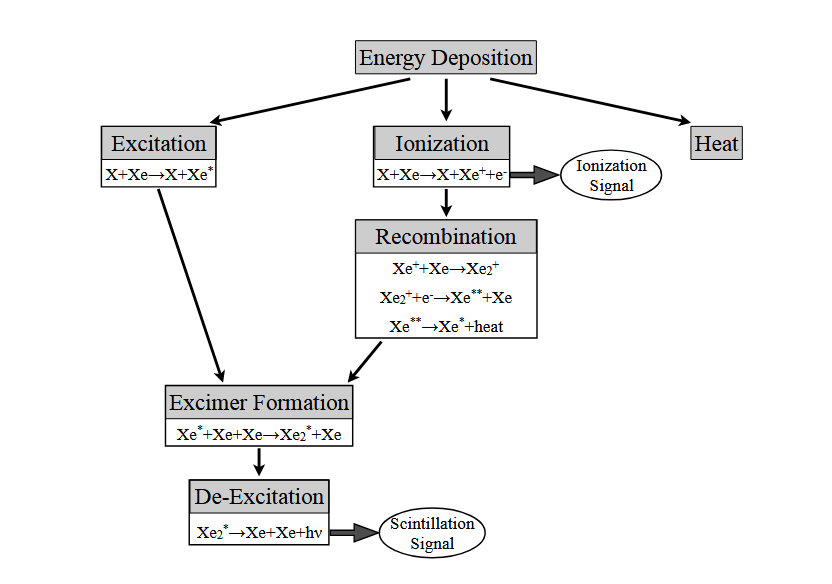
\includegraphics[width=0.45\textwidth]{pic/发光原理.png}
    \caption{氙发光原理示意图}
    \label{fig:setup2}
\end{figure}
闪烁光在气氙中的传播和散射过程对探测器的性能有着重要影响。由于氙气的受激能级大于对紫外光的吸收较弱，闪烁光能够在探测器内部高效地传播。然而氙的发光光谱与水，CO2,氧气等电负性气体吸收光谱重合因此，极微量的杂质也会显著降低光子的吸收效率，从而影响探测器的能量分辨。所以在设计气氙束流能损探测器时，需要特别注意探测器内部环境的清洁和稳定，确保氙气的高纯度，以最大程度地提升探测器的性能表现。
物理探测实验中来。PandaX 等暗物质探测实验合作组采用气液两相型 TPC,综合氙的闪
烁发光和电离特性进行暗物质探测[25]。在原子核物理探测领域，气氙探测器凭借其高
能量分辨率的优势和潜力也在 X 射线探测和𝛾𝛾射线测量方面被科学家们不断挖掘。
\section{探测器的光学蒙特卡洛模拟}

为了提升气氙束流能损探测器的工作能力，需要对探测器的设计进行优化。通过对探测器的光学蒙特卡洛模拟，可以评估不同设计方案的性能，并指导实际探测器的构建。蒙特卡洛模拟是一种基于随机数生成的数值方法，可以模拟粒子在探测器中的传播和相互作用过程，从而预测探测器的响应。本文采用Geant4(GEometry ANd Tracking)是由CERN(欧洲核子研究组织)基于C++面向对象技术开发的蒙特卡罗应用软件包，用于模拟粒子在物质中输运的物理过程。针对气氙的发光特性，本文主要通过模拟探测器中氙气的闪烁光的产生和传播过程，评估不同设计方案下探测器的能量分辨率和时间分辨率等性能指标。通过对模拟结果的分析，可以优化探测器的结构设计、材料选择、工作气压以及光电倍增管的布置，从而提升探测器在放射性束流能损测量中的性能表现。
\subsection{模型构建}
在Geant4中构建气氙束流能损探测器的模型，首先需要定义探测器的几何结构，包括探测器的尺寸、形状以及内部组件的布置。其次，需要设置探测器的材料属性，特别是氙气的物理和化学性质，如密度、原子序数、激发态能级等。然后，需要定义粒子源，即入射到探测器中的带电离子束流的能量分布、空间分布以及时间分布等参数。最后，需要设置探测器的响应机制，包括闪烁光的产生机制、光子的传播过程以及光电倍增管的响应特性等。通过以上步骤，可以构建一个完整的气氙束流能损探测器模型，为后续的蒙特卡洛模拟提供基础。

针对气束流激发氙闪烁发光过程，本项目采用的物理模型为FTFP\_BERT即强子物理模型，适用于高能粒子与物质的相互作用模拟。该模型结合了Fritiof模型（FTF）和Bertini级联模型（BERT），能够有效地模拟从几MeV到几TeV范围内的粒子与物质的相互作用过程。在模拟过程中，FTFP\_BERT模型可以准确地描述带电离子在氙气中的能量损失、激发态的产生以及闪烁光的发射过程，从而为评估探测器性能提供可靠的数据支持。此外，为了精准地模拟氙气紫外光的传播过程，还需要在Geant4中设置氙气的光学属性，如切伦科夫光、光子产额、发光时间常数、吸收长度等参数，以确保模拟结果能够真实反映探测器的实际性能表现。

\section{探测器主体设计}
根据蒙特卡洛模拟的结果，对探测器结构进行设计。




\clearpage

\chapter{探测器搭建和调试}
\section{气路系统}
为了保证气氙束流能损探测器的长期正常稳定工作，需要设计合理的气路系统和腔体结构。气路系统需要能够稳定地供应高纯度的氙气，并且能够有效地排除杂质和水分等污染物，以确保探测器内部环境的清洁和稳定。腔体结构需要具备良好的密封性能，能够承受一定的压力，并且能够有效地隔离外界环境对探测器内部的干扰。此外，腔体内部还需要设计合理的光学路径，以确保闪烁光能够高效地传输到光电倍增管上，从而提升探测器的响应效率和能量分辨率。在实际搭建过程中，还需要考虑到探测器的散热问题，确保探测器在长时间工作过程中能够保持稳定的温度，以避免因过热而导致性能下降或损坏。

探测器的气路系统主要分为真空，循环，纯化三个部分。真空系统主要用于抽取探测器内部的空气和杂质，确保探测器内部的清洁和稳定。循环系统主要用于将氙气在探测器内部循环流动，以保证氙气的均匀分布和稳定供应。纯化系统主要用于去除氙气中的杂质和水分等污染物，以确保探测器内部环境的清洁和稳定。在设计气路系统时，需要考虑到各个部分之间的连接方式、流量控制以及安全措施等方面，以确保整个系统能够高效、稳定地运行。为了避免腔体内油脂，在进行气路和腔体的组装过程中，对所有零部件进行严格的清洗和烘干处理，确保探测器内部环境的洁净和稳定。此外，在组装过程中还需要注意密封性能，确保腔体能够有效地隔离外界环境对探测器内部的干扰，从而提升探测器的性能表现。

气氙由99.999\%纯度的氙气瓶供应，经过纯化器后进入探测器内部循环使用。
探测器的循环部分由电磁泵实现，电磁泵具有无机械接触、无泄漏、无污染等优点，能够有效地提升探测器的性能表现。在实际搭建过程中，需要对电磁泵进行合理的安装和调试，以确保其能够高效、稳定地运行。通过控制电磁泵电源输入的电压及频率，可以很好的控制氙气的流速和流量。在安装前，通过流量计确定了流量，电压，频率的关系如下表所示：最终选定的工作点为电压为4.2V，频率为40Hz，此时流量为5nL/min，并且能够保持稳定的流速状态。实际工作过程中，还在电磁泵的旁路安装了500ml气罐作为buffer，能够有效地缓冲流量的波动，提升探测器的稳定性和性能表现。

探测器的纯化由纯化器实现。计划利用先普公司出产的纯化设备（Getter），在气体循环过程中利用高温锆吸附气体中存在的水和二氧化碳等杂质，从而保证氙中紫外光能够被光电倍增管接收到。该纯化器的工作温度为400℃，未工作时内部充满惰性气体Ar,能够有效地保护纯化器内部的活性材料不被氧化和污染。此外，气氙探测器还采用

在探测器工作前，需要保证气路的密封性和洁净度。首先将探测器由分子泵组抽真空至10$^{⁻5}$bar，并进行RGA（Residual Gas Analyzer，残余气体分析）分析，确认探测器内部的主要成分为氙气，并且杂质含量在可接受范围内。在分析过程中，发现气路系统中长期存在含量较高的水蒸气，为了减小水分对探测器性能的影响，在抽真空时缠绕加热带对清洗水蒸气较多的腔体等部位进行加热抽真空，极大的减小了气路内的水蒸气含量，以确保探测器内部环境的洁净和稳定。

此外，对探测器气路系统实施了氦质谱检漏：在气路接口处喷洒氦气，利用氦检仪监测氦气分压的变化。鉴于氦气分子直径最小、渗透性最强，是检测泄漏最灵敏的示踪气体，该方法可有效验证探测器的密封性能是否满足设计要求。

在确保探测器气路系统的密封性和洁净度后，通过依次开关气瓶和气路阀门，逐步引入氙气进入探测器内部，确保其符合设计要求。在引入氙气的过程中，还需要注意观察探测器内部的压力变化，直至满足工作气压。

\section{探测器腔体}
为适应束流探测以及闪烁光子收集的需求，需要对探测器的腔体进行一系列的测试。首先，探测器的束流窗口需要在保证密封性的同时具备足够的透过率，以确保入射粒子能够顺利进入探测器内部进行探测并减小能量损失。常见的放射性束流束斑直径约为8-10cm,实验的束流能区在200MeV/n-1000MeV/n，在前期模拟过程中，使用LISE++针对不同厚度的钛膜和特氟龙窗口，计算了它们对束流粒子能量损失的影响。结果表明，随着窗口厚度的增加，入射粒子的能量损失也随之增加，这可能会对探测器的能量分辨率产生不利影响。200um的钛膜窗口给束流能损造成的影响在1\%左右，因此本文采用了直径为10cm,厚度为20-200μm的金属钛膜和1mm的特氟龙(PTFE)作为窗口的备选材料进行一系列测试。
制作过程首先将两片CF100的法兰垫片夹上不同厚度的钛膜和特氟龙膜，中间依靠树脂胶水连接密封，并且在真空烘箱内加热至200$^{\circ}$C进行固化处理制作成为窗口安装至腔体上。

为了评估不同窗口的密封性能和强度，以保证其能承受在工作循环过程中产生的内外压强差以及保证探测器内部工作气体的稳定性。需要对不同厚度的钛膜和特氟龙膜进行压力测试，首先将探测器进行抽真空处理观察窗口的形变情况，结果发现在内外压差约为1atm时，20um的钛膜以及1mm的特氟龙膜均出现了较大的形变乃至彻底破损，无法满足探测器的需求。此外，束流窗口还需要保证较好的一致性，内外压差有波动时，能够保证其形状不发生明显变化，因此对探测器腔体进行了加压测试。通过对探测器内充入不同气压的Ar气体，利用激光测距仪测量不同位置点与测距仪的距离从而判断膜的形变窗口的形变情况。从表中可以看出，在抽真空后，Ti膜出现了较为明显的外凸现象，而随着内部气压的不断增加，Ti膜的形变逐渐减小，最大距离差在0.5mm左右，能够满足探测器的使用需求，且当内压达到4atm以上时，Ti膜依旧可以保证较好的一致性，证明其强度能够满足探测器在工作循环过程中产生的内外压强差以及保证探测器内部工作气体的稳定性的需求。

探测器腔体还需要满足良好的光学性能，以确保闪烁光能够高效地传输到光电倍增管上，从而提升探测器的响应效率和能量分辨率。根据上节的模拟结果，探测器的腔体内部加入了一个由PTFE制成的立方体PMT-holder，能够有效地反射闪烁光并将其引导到光电倍增管上，从而提升探测器的性能表现。

此外，为了实现腔体内部PMT的高压和信号的传输，腔体外部还设置了六个CF35接口，分别作为进出气口和高压信号的接口。其中进出气口转接为1/2VCR，能够满足探测器的气路连接需求；高压信号接口则采用了两个19pin的feedthrough，能够满足PMT的高压和信号传输需求。在实际搭建过程中，需要对这些接口进行合理的安装和调试，以确保其能够高效、稳定地运行，并且能够满足探测器的性能要求。具体信号电路设置见下一节PMT调试部分。一个CF35接口为真空测试接口，能够单独测试腔体的真空情况，便于测试。另设一个CF35接口作为观察窗口，能够通过安装一个透明的窗口来观察探测器内部的情况，以便于在调试和维护过程中进行监测和调整。
\section{PMT选型调试}
为了实现对探测器中闪烁光的高效检测，需要选择合适的光电倍增管（PMT）并进行调试。PMT的选择除了需要考虑其量子效率、增益、时间分辨率工作电压等参数，还需要针对束流探测器的特殊需求进行选择，如其在不同工作气压的气体中的稳定性、对辐射的耐受性等，以确保其能够满足探测器的性能要求。在实际调试过程中，需要对PMT进行合理的安装和连接，确保其能够与探测器的腔体和信号处理系统有效地配合工作。此外，还需要对PMT进行高压测试和信号测试，以验证其性能是否符合设计要求，并且能够在实际工作环境中稳定运行。通过对PMT的选型和调试，可以提升探测器对闪烁光的响应效率和能量分辨率，从而增强探测器在放射性束流能损测量中的性能表现。

由上节可知，气氙的闪烁光为在紫外光区域，波长约为175nm，常见的可见光区PMT对紫外光的量子效率较低，因此需要选择对紫外光具有较高量子效率的PMT。经过对各类参数的筛选，最终选定了Hamamatsu公司出产的R8520-406型号的PMT作为探测器的光电倍增管。
R8520探测器是一种多通道版PMT,具有增益高，量子效率高等优势。该型号PMT专门用于收集稀有气体Ar,Xe的闪烁光，广泛应用于暗物质探测等各类相关实验。其关键参数如下表所示
\begin{table}[htbp]
    \centering
    \begin{tabular}{cccc}
        \hline
        型号 & 波长范围 (nm) & 量子效率 (\%) & 工作电压 (V) \\
        \hline
        R8520-406 & 160-650 & 30 (175nm) & 800-1200 \\
        \hline
    \end{tabular}
    \caption{Hamamatsu R8520-406 PMT关键参数}
    \label{tab:PMT}
\end{table}
为了使PMT能够稳定工作并且实现稳定信号读出，需要针对本实验设计PMT的分压base电路。为了节省腔体空间，分压电路由PCB板实现，通过在PMT阳极上加上正高压实现光电子的倍增和加速。同时，考虑到16路高压和信号在feedthrough接口的传输需求，为了减小信号干扰和线路复杂度，采用了将信号和高压同时输出的设计方案：即信号和高压线在feedthrough接口处合并为一根线，在腔体外部通过加入滤波电容将高频信号和低频高压进行分离。用于
\clearpage

\chapter{气氙探测器测试}